\begin{sloppypar} % помогает в кириллическом документе выровнять текст по краям
\newpage % Так добавляется  новая страница

% \section*{ВВЕДЕНИЕ}%так объявляется новая глава. * означает, что эта глава не попадает в оглавление и не имеет номера.
% \addcontentsline{toc}{section}{\hspace{1mm}ВВЕДЕНИЕ} % эта строчка нужна, чтобы такую главу в оглавление все таки добавить, но без номера. Такие госты, что поделать.
% введение я вообще снес нахуй, так как не придумал, что там писать.

\section{Часть I} %Объявили начало главы
\subsection{Создание проекта и описание устройства с помощью VHDL} %Объявили начало раздела

По методике, описанной в методических указаниях к лабораторной работе, в программном пакете Vivado v2016.4 был создан проект.

Для описания портов и логики схемы используется файл с описанием устройства на языке VHDL \textit{fdc.vhd}, содержимое которого можно увидеть ниже:

% код можно вставить с помощью команды прямо из файла
\inputminted[
% frame=lines,%линия сверху и снизу блока кода
% framesep=15mm, % отступ между линией и кодом
baselinestretch=1, %интервал междустрочный
% bgcolor=LightGray, %цвет фона
fontsize=\footnotesize, %размер шрифта
% linenos%нумерация строк
]
{VHDL}%язык программирования
{fdc1.vhd}%файл с кодом(должен лежать в папке проекта)

Данный код описывает в одном модуле всю схему, представленную на
рисунке 1. Первый блок \textit{process (C)} описывает логику D-триггеров DD1 и
DD2. Второй блок \textit{process (C) }– логику конъюнктора DD3 и D-триггера DD4.

% код так же можно вставить вот так, прямо кодом, не через файл.
% \begin{minted} [
% frame=lines,%линия сверху и снизу блока кода
% framesep=15mm, % отступ между линией и кодом
% baselinestretch=1, %интервал междустрочный
% bgcolor=LightGray, %цвет фона
% fontsize=\footnotesize, %размер шрифта
% linenos%нумерация строк
% ]{VHDL}
% library IEEE;
% use IEEE.STD_LOGIC_1164.ALL;

% entity fdc is 
    % Port (D_0, D_1: in STD_LOGIC;
    % C : in STD_LOGIC;
    % Q : out STD_LOGIC);
% end fdc;

% architecture Behavioral of fdc is

% signal x_0, x_1 : STD_LogIC;
    
% begin
    % process (C)
    % begin
        % if rising_edge(C) then
        % X_0 <= D_0;
        % X_1 <= D_1;
    % end if;
% end process;
    % process (C)
    % begin
        % if rising_edge(C) then
        % Q<= X_0 and X_1;
        % end if;
    % end process;
% end Behavioral;
% \end{minted}

% С кодом разобрались, окей
\subsection{Симуляция устройства} %Объявили начало раздела
Следующий этап - симуляция устройства на поведенческом уровне. В данном этапе мы уже можем наблюдать, как работает логика описанного устройства, но пока без учета физических особенностей микросхемы.
Для этого был создан файл симуляции (Test bench) tb\_sim.vhd на языке VHDL, содержимое которого можно увидеть ниже:
\inputminted[
% frame=lines,%линия сверху и снизу блока кода
% framesep=15mm, % отступ между линией и кодом
baselinestretch=1, %интервал междустрочный
% bgcolor=LightGray, %цвет фона
fontsize=\footnotesize, %размер шрифта
% linenos%нумерация строк
]
{VHDL}%язык программирования
{tb_sim1.vhd}%файл с кодом(должен лежать в папке проекта)

После запуска симуляции были получены временные диаграммы, изображенные на рисунке \ref{ris:Figures/2022-10-10_22-59-24.png}.

\imgh{160.5mm}{Figures/2022-10-10_22-59-24.png}{Результат симуляции} %можно так вставить изображение


% так, с изображением разобрались, есть еще такой способ, с одной стороны чуть более гибкий, с другой - длиннее код
% \begin{figure}[!htb]
	% \centering
	% 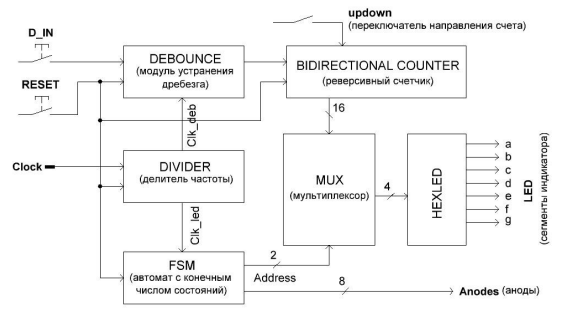
\includegraphics[width=\textwidth]{Figures/2022-10-10_22-59-24.png}
	% \caption{Здесь может быть указана подпись рисунка}\label{fig:Figures/2022-10-10_22-59-24.png}
% \end{figure}
% Параметр width задаёт ширину рисунка. В этом случае она равна ширине текста, \textwidth. Вместо \textwidth можно укзать значение от 0.1 до 1. \label нужен для того, чтобы потом можно делать сноску на эту картинку, как было выше(ну где  написано типа \ref{ris:Figures/2022-10-10_22-59-24.png}.)

\newpage % ебанем новую страницу
\subsection{Синтез цифрового устройства} %Объявили начало раздела
\subsubsection{Схема цифрового устройства} %Объявили начало подраздела

После формального описания устройства с помощью VHDL, и запуска симуляции на поведенческом уровне приступают к синтезу устройства. Открыв в окне Flow Navigator спойлер RTL analysis, выбрав в нем пункт /Elaborated Design/Schematic, можно увидеть схему, которую пакет Vivado синтезировал на основе текстового описания(рисунок \ref{ris:Figures/2022-10-20_00-24-24.png})

\imgh{160.5mm}{Figures/2022-10-20_00-24-24.png}{Синтезированная c помощью RTL Analysis схема}

Можно заметить, что полученная схема ничем не отличается от принципиальной схемы из методических указаний к лабораторной работе(рисунок \ref{ris:Figures/2022-10-11_20-10-59.png})
\imgh{160.5mm}{Figures/2022-10-11_20-10-59.png}{Принципиальная схема из методических указаний к лабораторной работе}

Запуская синтез проекта, пакет Vivado получает задание сформировать на основе текстового описания устройства список соединений(Netlist), который будет использован для размещения всей логики схемы внутри ПЛИС, то есть перейти от абстрактного описания устройства к модели, учитывающей физические особенности микросхемы. На данном этапе необходимо провести тщательный временной анализ, необходимый для обнаружения узких мест и обеспечения эффективной и надежной работы устройства. 

В результате синтеза была получена следующая схема (рисунок \ref{ris:Figures/2022-10-11_19-48-02.png})


\imgh{160.5mm}{Figures/2022-10-11_19-48-02.png}{Синтезированная схема}
От принципиальной схемы, изображенной в методических указаниях в начале работы (рисунок \ref{ris:Figures/2022-10-11_20-10-59.png}), полученная в результате синтеза схема отличается наличием буферных каскадов IBUF и OBUF(вероятно, это сокращения от input и output buffer), по всей видимости необходимых для согласования напряжений внутри и снаружи микросхемы, согласования сопротивлений.. Так же отличием можно считать элемент BUFG, который нужен, как я понял, для того, чтобы использовать глобальный тактовый сигнал. Так же каждый из D-триггеров на синтезированной схеме имеет неиспользуемый заземленный вход CE(clock enabled). Все это лишь технические особенности проектирования, и на функциональность устройства влияние не оказывает.
\newpage
\subsubsection{Временные ограничения} %Объявили начало подраздела

Полученный в прошлом этапе нетлист анализируется временным анализатором для расчета длительности передачи данных внутри ПЛИС. Эти длительности должны лежать во вполне определенных пределах, диктуемых физическими параметрами микросхемы. Внутренние задержки, присущие элементам ПЛИС, такие как \begin{math}t_{SETUP}\end{math}  и \begin{math}t_{HOLD}\end{math}, пакету Vivado известны. Параметры внешних устройств необходимо задать вручную, используя справочные данные.

Проделав описанные в методических указаниях шаги, получены следующие результаты(рисунок \ref{ris:Figures/2022-10-11_22-17-53.png})
\imgh{160.5mm}{Figures/2022-10-11_22-17-53.png}{Total Negative Slack}

Просмотрев подробный отчет, можно увидеть, что задержка установления образуется на выходе, по пути через D-триггер DD4, и output buffer (рисунок \ref{ris:Figures/2022-10-20_04-19-58.png})
\imgh{160.5mm}{Figures/2022-10-20_04-19-58.png}{путь, в котором образуется задержка установления} 

Можно увидеть, что проблемы с временем удержания кроются в пути от входов D\_0 и D\_1 (рисунок \ref{ris:Figures/2022-10-20_04-19-59.png})
\imgh{160.5mm}{Figures/2022-10-20_04-19-59.png}{путь, в котором образуется задержка удержания}

На рисунке \ref{ris:Figures/2022-10-20_04-19-57.png} показан отчет по времени установления для пути с наибольшей задержкой.
\imgh{80.5mm}{Figures/2022-10-20_04-19-57.png}{отчет по времени установления}

Решить эти проблемы предлагалось с помощью уменьшения частоты схемы. Увеличив период тактового сигнала с 5 до 8 нс, в результате повторного синтеза были получены следующие результаты(рисунок \ref{ris:Figures/2022-10-11_22-17-3.png})

\imgh{160.5mm}{Figures/2022-10-11_22-17-3.png}{Total Negative Slack равен нулю, и есть даже небольшой запас в 0.151ns}

\imgh{80.5mm}{Figures/2022-10-20_04-51-55.png}{время установления после уменьшения частоты схемы}


Согласно методическим указаниям, решить проблему с временем удержания можно будет в следующем разделе.

\newpage
\subsection{РЕАЛИЗАЦИЯ} %Объявили начало раздела
Следующий шаг разработки устройства – это реализация. Для размещения схемы внутри ПЛИС необходимо выбрать внешние выводы для подключения входов и выходов устройства. Это может делаться разработчиком из
конструктивных соображений, либо возможен вариант авторазмещения, когда Vivado автоматически назначает внешние выводы. В нашем случае целесообразно воспользоваться именно авторазмещением

\imgh{120.5mm}{Figures/2022-10-20_05-12-48.png}{Фрагмент карты доступных контактов}

После реализации устройства снова появились проблемы с временем установления, в то время как проблемы с временем удержания исчезли.

\imgh{80.5mm}{Figures/2022-10-20_05-12-8.png}{Очередные проблемы с временем установления}

Предложенный в методических указаниях способ с помощью выбора стратегии реализации не помог решить указанную проблему. В итоге, период пришлось увеличить с 8 до 12 нс. 
\newpage
\subsection{Индивидуальные задания}%такая глава попадает в оглавление и имеет номер.
1. Выясните, какая максимальная частота работы схемы возможна при заданных временных ограничениях.

Как было указано выше, при заданных временных ограничениях схема реализуется при частоте  	\begin{displaymath}\nu=\frac{1}{T}=\frac{1}{12*10^{-9}}=83*10^6 Гц\end{displaymath}


2. Выберите ПЛИС с другими параметрами (опции -2 или -3 в названии) и определите, какая максимальная частота возможна для них.

Не совсем понял формулировку задания про опции

3. Установите вручную положение вывода Clock на E3 и заставьте Vivado автоматически разместить все остальные выводы.
\imgh{160.5mm}{Figures/2022-10-20_05-12-8111.png}{Вручную расположен вывод Clock и автоматически размещены остальные выводы}
% \imgh{160.5mm}{Figures/2022-10-20_05-12-111.png}{Вручную расположен вывод Clock и автоматически размещены остальные выводы}

4. Вернитесь к этапу моделирования и повторите его используя «Run Post-Synthesis Functional Simulation», «Run Post-Synthesis Timing Simulation», «Run Post-Implementation Functional Simulation» и «Run Post-Implementation Timing Simulation». Сравните полученные результаты с результатами, полученными в разделе 2.

\imghh{160.5mm}{Figures/2022-10-20_07-13-49.png}{Run Behavioral Simulation}
\imghh{160.5mm}{Figures/2022-10-20_07-18-05.png}{Run Post-Synthesis Functional Simulation}
\imghh{160.5mm}{Figures/2022-10-20_07-19-58.png}{Run Post-Synthesis Timing Simulation}
\imghh{160.5mm}{Figures/2022-10-20_07-40-02.png}{Run Post-Implementation Functional Simulation}
\imghh{160.5mm}{Figures/2022-10-20_07-41-42.png}{Run Post-Implementation Timing Simulation}

Behavioral Simulation и Run Post-Synthesis Functional Simulation - разница в начальный момент времени. В Behavioral в начальный момент времени на выходе  неопределенное состояние, после синтеза в начальный момент времени на выходе 0. В обоих симуляциях типа Timing на выходе сигнала не наблюдается...

5. Повторите пункт 4, задав другую частоту тактового сигнала.
С частотой 50 МГц: 
\imghh{160.5mm}{Figures/beh_50mhz.png}{Run Behavioral Simulation}
Остальные файлы добавлять смысла нет, общая картина повторяет предыдущий пункт.

6. Добавьте к наблюдаемым сигналам внутренние сигналы (выходы элемента «И» и триггеров первой ступени) и посмотрите, как выполняются временные соотношения

Не совсем понял, как добавить  внутренний сигнал - выход элемента «И». (рисунок \ref{ris:Figures/scopes.png}). Предлагается по умолчанию вывести состояние входов и выходов, так же можно вывести внутренние сигналы, объявленные в fdc.vhd, но сигнал Q с точки зрения кода это и есть то, что на выходе элемента "И". 

\imghh{160.5mm}{Figures/scopes.png}{объекты для которых можно вывести на экран}
%https://russianblogs.com/article/24401675772/ по идее тут про это все написано




\section*{ОТВЕТЫ НА ВОПРОСЫ ДЛЯ САМОПРОВЕРКИ}
\addcontentsline{toc}{section}{\hspace{1mm}ОТВЕТЫ НА ВОПРОСЫ ДЛЯ САМОПРОВЕРКИ}

\textit {1. Какие два подхода к описанию аппаратуры вы знаете? Какой подход
вы использовали в лабораторной работе?}

Используют графический способ(где по необходимой логической функции рисуют структурную схему), или же описательный(текстовый), с помощью языков описания аппаратуры. В лабораторной работе использовался преимущественно второй способ, хотя и графическая схема была синтезирована.

\textit {2. Какие языки описания аппаратуры (HDL) вы знаете? Какой язык вы
использовали в лабораторной работе?}

Наиболее известные языки описания аппаратуры  - VHDL, Verilog, SystemVerilog. В лабораторной работе использовался VHDL.

\textit {3. Какой программный пакет и какую ПЛИС вы использовали в лабораторной работе?}

Программный пакет Vivado v2016.4 и ПЛИС Artix-7, в составе отладочной платы Nexys-4

\textit {4. Опишите стандартный процесс проектирования цифровых устройств.}

Формализация логики устройства с помощью логического выражения, затем описание этой логики с помощью текстового описания или графически, симуляция на поведенческом уровне, синтез устройства, реализация устройства, отладка.

\textit {5. Вспомните таблицу переходов D-триггера и таблицу истинности логического вентиля И.}
\imgh{80.5mm}{Figures/2022-10-20_05-12-811.png}{Таблица переходов D-триггера и таблица истинности логического вентиля И.}

\textit {6. Для чего нужна симуляция устройства на поведенческом уровне?}

Для проверки функционирования устройства на уровне логики, без учета физических задержек.

\textit {7. Для чего необходимо задавать временные задержки?}

Чтобы не допустить метастабильности, и как следствие, сбоев и ошибок в работе, которые появятся, если не учесть задержки в нужных местах.

\textit {8. На каком этапе проектирования цифровых устройств строится топология проекта и подключаются внешние выводы?}

На этапе синтеза это происходит формально(описываются выводы, задаются для них параметры задержек, а так же определяют местоположение выводов на ПЛИС)
Вообще это вполне тянет на отдельный этап проектирования. В рамках лабораторной работы это происходилов в момент синтеза.

\textit {9. Опишите назначение строк кода в файле fdc.vhd.}
% код можно вставить с помощью команды прямо из файла
\inputminted[
% frame=lines,%линия сверху и снизу блока кода
% framesep=15mm, % отступ между линией и кодом
baselinestretch=1, %интервал междустрочный
% bgcolor=LightGray, %цвет фона
fontsize=\footnotesize, %размер шрифта
% linenos%нумерация строк
]
{VHDL}%язык программирования
{fdc.vhd}%файл с кодом(должен лежать в папке проекта)


\textit {10. Опишите назначение строк кода файла симуляции tb\_sim.vhd.}
% код можно вставить с помощью команды прямо из файла
\inputminted[
% frame=lines,%линия сверху и снизу блока кода
% framesep=15mm, % отступ между линией и кодом
baselinestretch=1, %интервал междустрочный
% bgcolor=LightGray, %цвет фона
fontsize=\footnotesize, %размер шрифта
% linenos%нумерация строк
]
{VHDL}%язык программирования
{tb_sim.vhd}%файл с кодом(должен лежать в папке проекта)

\textit {11. Нарисуйте временную диаграмму работы вашего устройства и сравните ее с диаграммой, полученной в результате симуляции.}


\textit {12. Что такое ограничения проектирования и для чего они нужны?}

Ограничения вызваны законами физики.  Это и ограничения по напряжениям и токам, и ограничения скорости распространения сигналов, и многое другое. Учесть их -- задача инженера, ведь, будучи учтенными, они не помешают работе устройства. 

\textit {13. Какие временные ограничения вы задавали в вашем проекте?}

В проекте задавались временные ограничения для внешних устройств, подключаемых  к ПЛИС



% \newpage
% \bibliographystyle{plain}
% \bibliography{bibliography}


\end{sloppypar}
